\documentclass[12pt]{article}

\usepackage[margin=1in]{geometry}
\usepackage{amsmath,amsfonts,amssymb}
\usepackage{graphicx}
\usepackage{cite}
\usepackage{hyperref}
\usepackage{physics}
\usepackage{caption}
\usepackage{booktabs}
\usepackage{setspace}
\usepackage{tikz}
\usepackage{titlesec}
\usepackage[verbose]{placeins}

\titleformat{\section}{\large\bfseries}{\thesection.}{0.5em}{}
\titleformat{\subsection}{\normalsize\bfseries}{\thesubsection.}{0.5em}{}

\title{\textbf{Finite Difference Time Domain Method for Computational Electromagnetics}}
\author{C2C Ethan Chapman \\ ECE 343}
\date{}

\begin{document}

\maketitle
\begin{spacing}{1.5}

\section{Introduction}
Maxwell's equations govern all classical electromagnetic phenomena. Analytical solutions are only feasible for a limited number of idealized problems. To address complex geometries and inhomogeneous media, computational methods are necessary. Several approaches exist, including the Finite Element Method (FEM), Method of Moments (MoM), and the Finite Difference Time Domain (FDTD) method. FDTD stands out for its explicit time-stepping scheme and intuitive grid-based implementation, making it especially useful for visualizations.

\section{Maxwell's Equations}
Maxwell's equations form the foundation of classical electromagnetics. They describe how electric and magnetic fields propagate and interact with charges and currents. These equations are expressed both in integral and differential (point) forms.

\FloatBarrier

\begin{table}[h!]
\centering
\renewcommand{\arraystretch}{2.0}
\begin{tabular}{|c|c|}
\hline
\textbf{Integral Form} & \textbf{Point Form} \\
\hline
$\displaystyle \iint \epsilon \vec{E} \cdot d\vec{S} = Q_{\text{enc}}$ 
& 
$\displaystyle \nabla \cdot \vec{E} = \frac{\rho_v}{\epsilon}$ \\
\hline
$\displaystyle \iint \vec{H} \cdot d\vec{S} = 0$ 
& 
$\displaystyle \nabla \cdot \vec{H} = 0$ \\
\hline
$\displaystyle \oint_C \vec{E} \cdot d\vec{\ell} = -\frac{d\Psi_m}{dt}$ 
& 
$\displaystyle \nabla \times \vec{E} = -\mu \frac{\partial \vec{H}}{\partial t}$ \\
\hline
$\displaystyle \oint_C \vec{E} \cdot d\vec{\ell} = - \iint \frac{\partial \vec{B}}{\partial t} \cdot d\vec{S}$ 
& 
\\
\hline
$\displaystyle \oint_C \vec{H} \cdot d\vec{\ell} = I_{\text{encl}}$ 
& 
\\
\hline
$\displaystyle \oint_C \vec{H} \cdot d\vec{\ell} = \int \vec{J} \cdot d\vec{S} + \epsilon \frac{\partial}{\partial t} \int \vec{E} \cdot d\vec{S}$ 
& 
$\displaystyle \nabla \times \vec{H} = \sigma \vec{E} + \epsilon \frac{\partial \vec{E}}{\partial t}$ \\
\hline
\end{tabular}
\caption{Maxwell’s Equations in Integral and Point Form}
\end{table}

\FloatBarrier

\section{Finite Difference Time Domain (FDTD) Method}
\subsection{Overview}
The Finite Difference Time Domain (FDTD) method is a time-domain numerical method that directly solves Maxwell's curl equations using finite-difference approximations. Fields are computed at discrete points in space and updated at successive time steps. 

\subsection{The Yee Cell}
The Yee cell, which staggers electric and magnetic field components in space and time, is used to model each distinct part of space during the simulation. The electric field components are at on edges of the cell and the magnetic field components are at the center of each face of the cell.

\begin{figure}
	\centering
	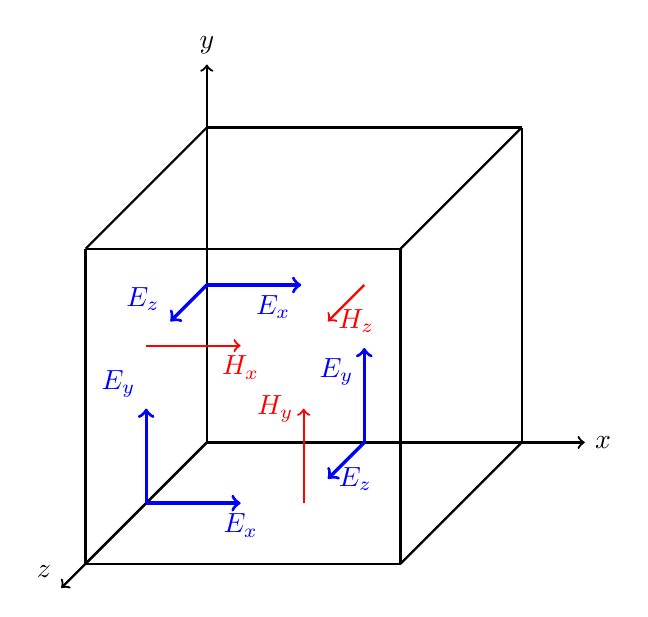
\begin{tikzpicture}[scale=4, thick]
	
	% Draw cube
	\draw[->] (0,0,0) -- (1.2,0,0) node[right] {$x$};
	\draw[->] (0,0,0) -- (0,1.2,0) node[above] {$y$};
	\draw[->] (0,0,0) -- (0,0,1.2) node[above left] {$z$};
	
	% Edges of the cube
	\draw (0,0,0) -- (1,0,0);
	\draw (0,0,0) -- (0,1,0);
	\draw (0,0,0) -- (0,0,1);
	\draw (1,0,0) -- (1,1,0);
	\draw (1,0,0) -- (1,0,1);
	\draw (0,1,0) -- (1,1,0);
	\draw (0,1,0) -- (0,1,1);
	\draw (0,0,1) -- (1,0,1);
	\draw (0,0,1) -- (0,1,1);
	\draw (1,1,0) -- (1,1,1);
	\draw (1,0,1) -- (1,1,1);
	\draw (0,1,1) -- (1,1,1);
	
	% E fields
	\draw[->,blue,very thick] (0.5,0,0) -- +(0,0.3,0) node[below left] {$E_y$};
	\draw[->,blue,very thick] (0,0.5,0) -- +(0.3,0,0) node[below left] {$E_x$};
	\draw[->,blue,very thick] (0,0,0.5) -- +(0.3,0,0) node[below] {$E_x$};
	\draw[->,blue,very thick] (0,0.5,0) -- +(0,0,0.3) node[above left] {$E_z$};
	\draw[->,blue,very thick] (0.5,0,0) -- +(0,0,0.3) node[right] {$E_z$};
	\draw[->,blue,very thick] (0,0,0.5) -- +(0,0.3,0) node[above left] {$E_y$};
	
	% H fields
	\draw[->,red,thick] (0.5,0.5,0) -- +(0,0,0.3) node[right] {$H_z$};
	\draw[->,red,thick] (0.5,0,0.5) -- +(0,0.3,0) node[left] {$H_y$};
	\draw[->,red,thick] (0,0.5,0.5) -- +(0.3,0,0) node[below] {$H_x$};
	
	\end{tikzpicture}
    \caption{The Yee cell.}
\end{figure}

\FloatBarrier

\subsection{Update Equations}

FDTD uses the two following point form equations we learned during class:

\begin{align}
\nabla \times \vec{E} &= -\mu \frac{\partial \vec{H}}{\partial t} \\
\nabla \times \vec{H} &= \epsilon \frac{\partial \vec{E}}{\partial t} + \vec{J}
\end{align}

Multiplying both sides by a small time step yields (approximately):

\begin{align}
\Delta t(\nabla \times \vec{E}) &= -\mu \Delta \vec{H} \\
\Delta t(\nabla \times \vec{H}) &= \epsilon \Delta \vec{E}
\end{align}

Now solving for the change in each field:

\begin{align}
\Delta\vec{E} &= \frac{\Delta t}{\epsilon} (\nabla \times \vec{H}) \\
\Delta\vec{H} &= -\frac{\Delta t}{\mu} (\nabla \times \vec{E})
\end{align}

Updating the magnetic field on each half-step we now have our FDTD update equations:

\begin{align}
\vec{E}^{n+1} &= \vec{E}^n + \frac{\Delta t}{\epsilon} (\nabla \times \vec{H}^n) \\
\vec{H}^{n+1/2} &= \vec{H}^{n-1/2} - \frac{\Delta t}{\mu} (\nabla \times \vec{E}^n)
\end{align}

\subsection{Basic Implementation Pseudocode}
\begin{verbatim}
Initialize E and H fields to zero
For each time step:
    Update H using curl of E
    Update E using curl of H
    Apply sources
    Apply boundary conditions
\end{verbatim}

\subsection{Advantages}
FDTD is straightforward to implement. The algorithm relies only on the values at nearby grid points, enabling efficient and explicit time stepping. Additionally, it supports wideband simulations since all frequencies are captured during time-domain evolution, making it particularly suited for pulsed or transient sources. Additionally, it is very easy to visualize and much easier to understand when compared to frequency-domain methods of computational electromagnetics.

\subsection{Limitations}
The main constraint in FDTD is the Courant-Friedrichs-Lewy (CFL) condition:

\begin{align}
	\frac{c \Delta t}{\Delta x} \leq 1
\end{align}

This condition ensures stability but limits the time step, particularly in high-resolution simulations. Additionally, memory usage scales quickly with domain size and resolution, making large simulations computationally intensive.

\section{2D Simulation}
A 2D FDTD simulation can model the propagation of a uniform plane wave in free space or through materials. The simulation space is discretized into a grid, and a Gaussian source is introduced. The electric field ($E_z$) and magnetic fields ($H_x$, $H_y$) evolve over time based on the update equations.

This setup is ideal for visualizing wave propagation and interactions with boundaries or materials. Parameters such as time step and spatial resolution must be chosen to satisfy the CFL condition and ensure sufficient resolution. Simulation was done using MATLAB, with code borrowed from \cite{ece6340lecture14} and enhanced to allow 2D simulation and objects in the simulation space. For all simulation pictures the electric field intensity is mapped to the red channel of each pixel and the magnetic field intensity is mapped to the blue channel of each pixel.


\subsection{Basic Wave Propogation}

The first simulation that was created showcases how the wave resulting from a Gaussian source propogates through free space. It is shown below:

\begin{figure}[h!]
    \centering
    
\includegraphics[width=0.5\textwidth]{sim0}
    \caption{Gaussian source propogating through free space.}
    \label{fig:sim0}
\end{figure}

\FloatBarrier

Once this wave reaches the edge of our simulation space it is reflected back. The result of that is shown below:

\begin{figure}[h!]
    \centering
    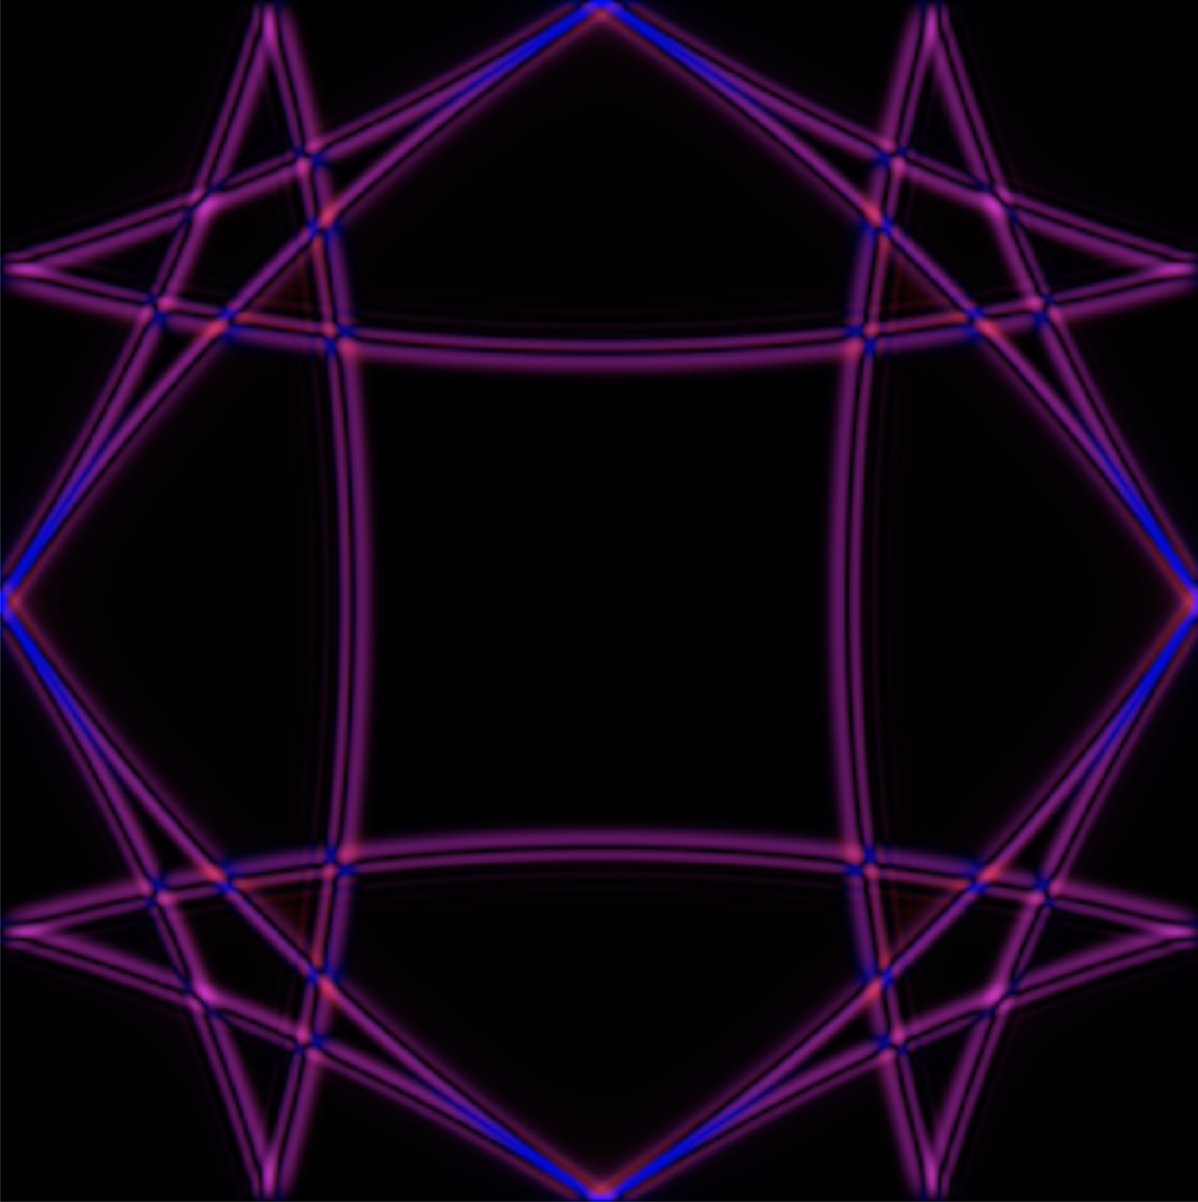
\includegraphics[width=0.5\textwidth]{sim1}
    \caption{Reflections at the boundary.}
    \label{fig:sim1}
\end{figure}

\FloatBarrier

\section{Objects in the Simulation Space}
FDTD simulations can include embedded objects by modifying the material parameters $\epsilon$, $\mu$, and $\sigma$ within specific grid regions. For instance, assigning a higher $\epsilon$ models a dielectric, while $\sigma > 0$ introduces a lossy material. Metal objects are simulated using perfect electrical conductor (PEC) conditions, setting electric fields to zero within the region.

Objects cause partial reflection, refraction, or absorption, depending on their material properties and geometry. This allows modeling of waveguides, resonators, scatterers, and more.

\begin{figure}[h!]
    \centering
    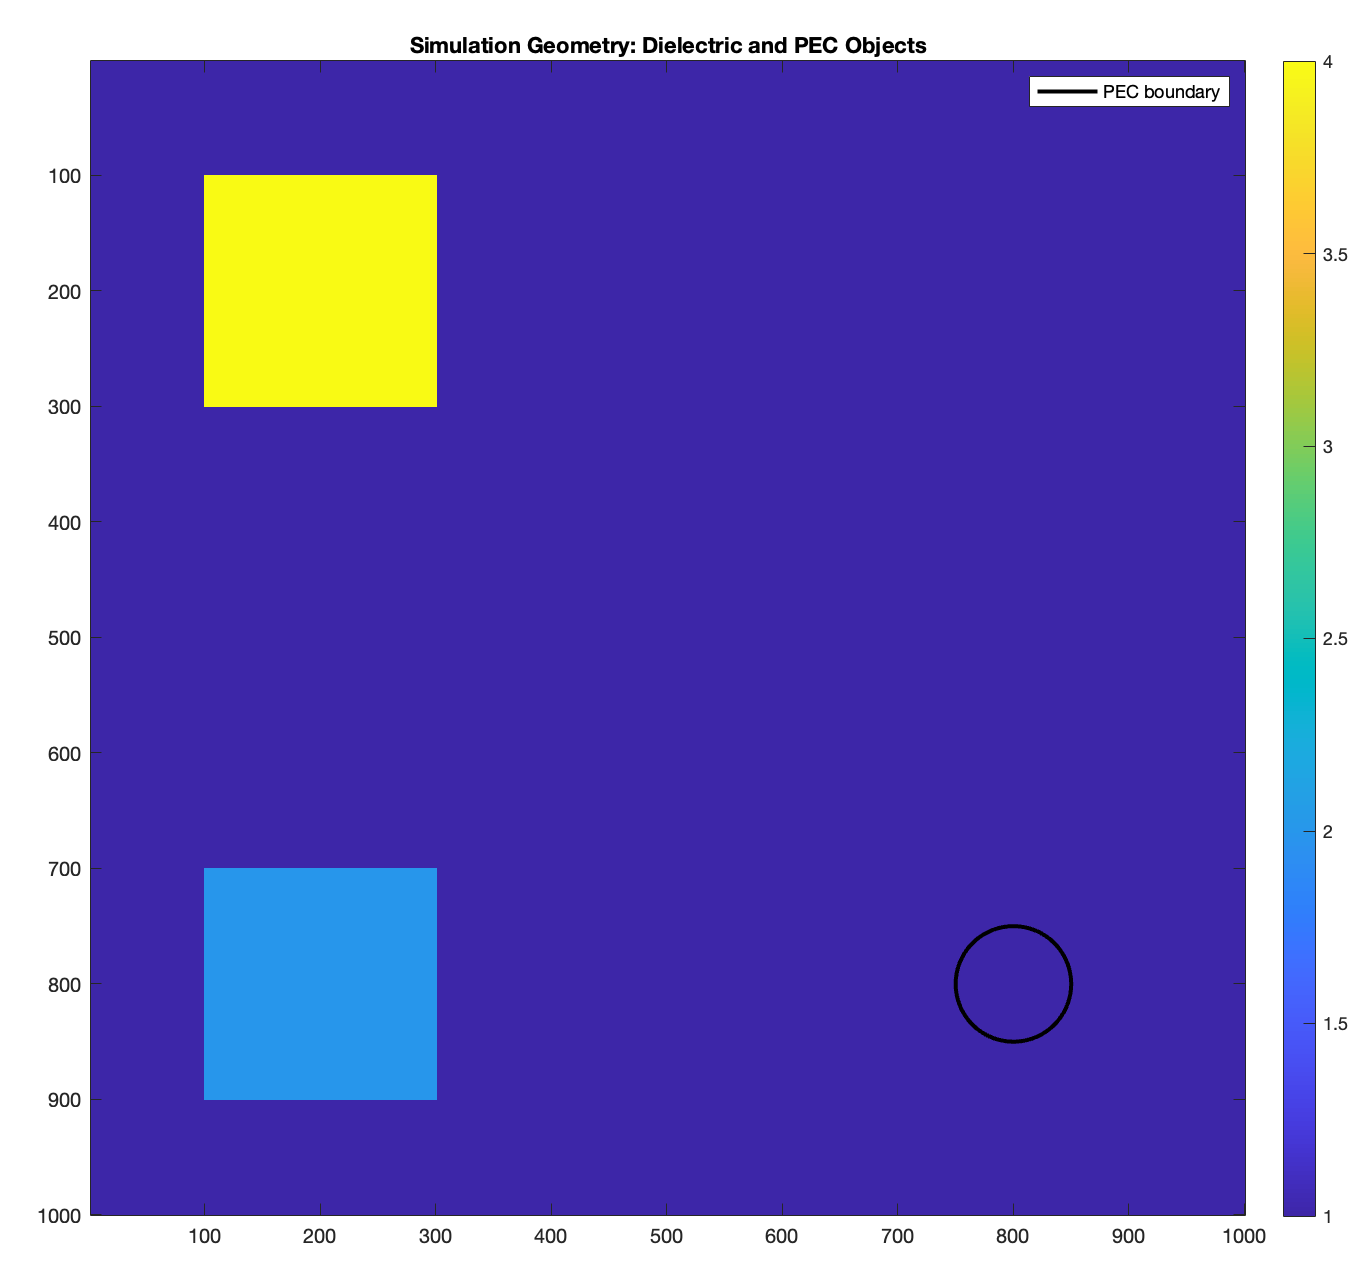
\includegraphics[width=0.75\textwidth]{sim_geom}
    \caption{Simulation layout with dielectric and PEC objects.}
    \label{fig:sim_geom}
\end{figure}

\begin{figure}[h!]
    \centering
    
\includegraphics[width=0.5\textwidth]{sim2}
    \caption{Initial field interaction with objects.}
    \label{fig:sim2}
\end{figure}

\FloatBarrier

Above we can see the wave's initial interaction with each object. On the top right, it is passing through a dielectric material with $\mu = 4$. We can see that the wave slows down and it's angle changes as we'd expect. On the bottom left, the same thing is happening but through a material with $\mu = 2$. Therefore, the distortions to the wave are occuring at a lesser degree. On the bottom right, the wave is being reflected off of the PEC. We can let this simulation keep running and observer the end state (not stable):

\begin{figure}[h!]
    \centering
    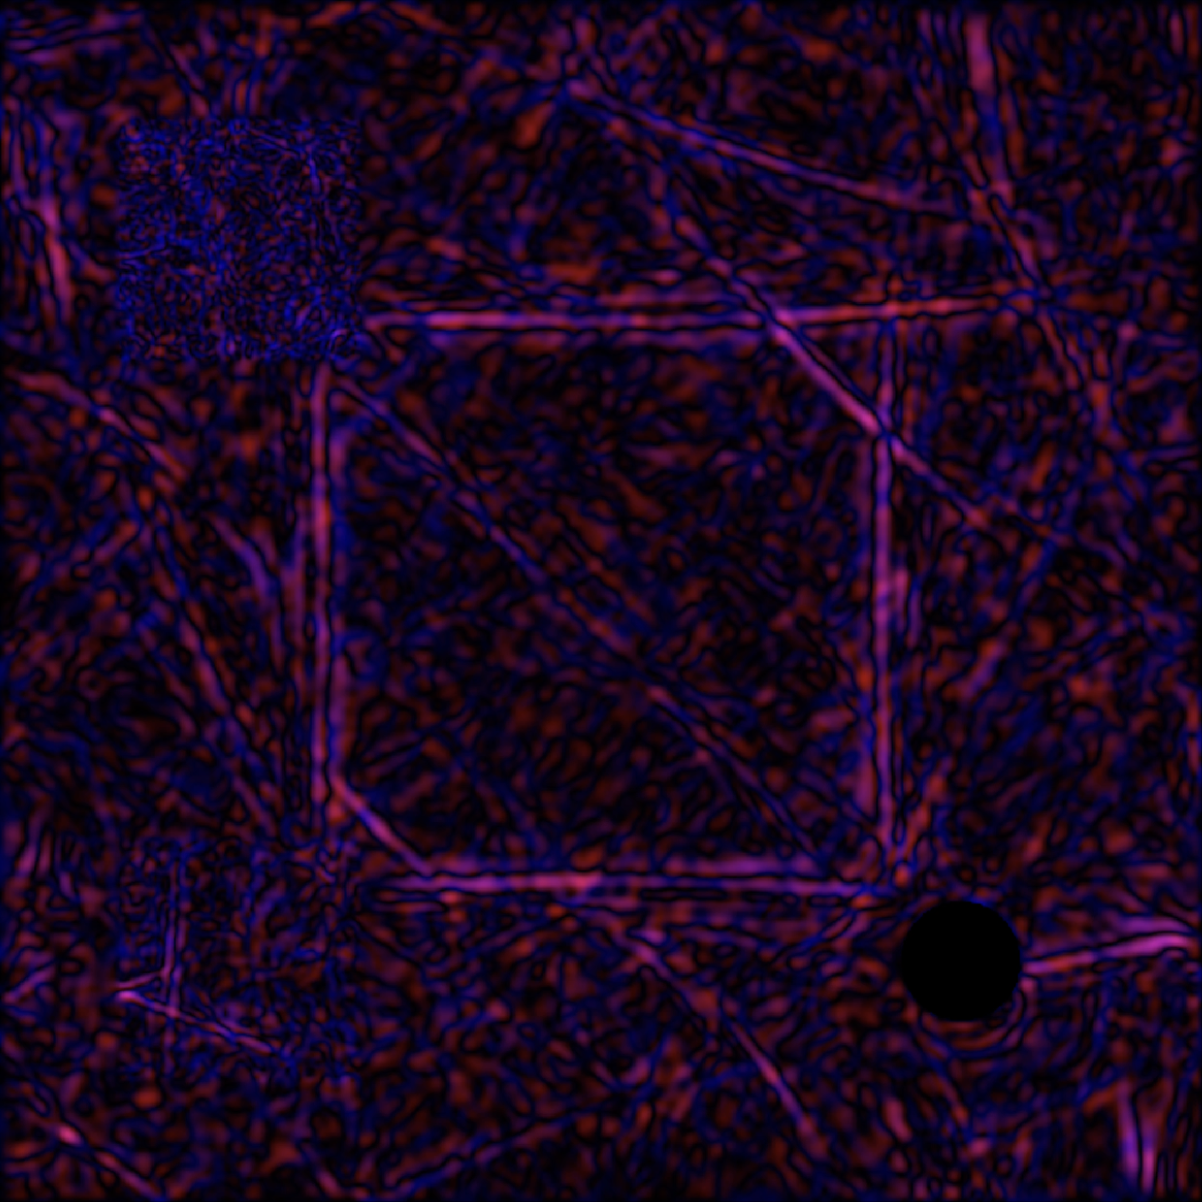
\includegraphics[width=0.5\textwidth]{sim3}
    \caption{End-state field interaction with objects.}
    \label{fig:sim3}
\end{figure}

\FloatBarrier

\section{Animated Simulations}

Animated simulations can be found in this GitHub repository: 


\bibliographystyle{IEEEtran}
\bibliography{cem_refs}

\end{spacing}
\end{document}
